\subsubsection{\stid{4.05} STDM07-VeloC: Very Low Overhead Transparent Multilevel Checkpoint/Restart} 

\paragraph{Overview} 

The VeloC project aims to provide a high-performance, scalable
checkpoint/restart framework that leverages multi-level checkpointing
(the combination of several resilience strategies and heterogeneous
storage) to ensure that ECP applications run to completion with
minimal performance overhead. It delivers a production-ready solution
that increases development productivity by reducing the complexity of
having to deal with a heterogeneous storage stack and multiple vendor
APIs. VeloC offers a client library that can be used by the
applications to capture local application states, which are then
coordinated and persisted using a resilience engine. The VeloC
software intends to serve ECP applications such as HACC, NWChemEx,
LatticeQCD and EXAALT.

\paragraph{Key Challenges}

Applications typically employ simple checkpoint-restart mechanisms to
survive failures that directly use a parallel file system.  However,
I/O bottlenecks due to concurrent writes are a known limitation in
this case. At Exascale, I/O bottlenecks are amplified both because
failures happen more frequently and because I/O bandwidth per compute
unit decreases (high increase in compute capability, modest increase
in I/O capability). Therefore, simple checkpoint-restart mechanisms
are not feasible. To compensate for the decreasing I/O bandwidth per
compute unit, the storage stack is becoming increasingly more
heterogeneous (e.g. NVRAM, burst buffers, key-value stores,
etc.). This aspect introduces a new level of complexity for
application developers: they need to adapt their checkpoint strategy
to a variety of new storage sub-systems that may or may not be
available on every machine. This is further amplified by the diversity
of vendors that offer custom APIs. Thus, it is important to provide a
scalable high-performance checkpointing solution that can leverage the
heterogeneous storage stack transparently without sacrificing ease of
use and flexibility.

\paragraph{Solution Strategy}

To address these challenges, VeloC is based on several design principles.

First, it implements multi-level checkpointing. Specifically, it
persists the local checkpoints to other nodes using collaborative
resilience strategies (e.g., partner replication and partner erasure
coding) and to external storage that may include a complex
heterogeneous hierarchy (e.g., parallel file system, burst buffers,
I/O nodes, key-value stores, etc.). Based on experience from previous
efforts such as FTI~\cite{FTI} and SCR~\cite{SCR}, this strategy
greatly improves performance and scalability.

Second, it offers a simple API that enables users to either manually
capture checkpoints into files or to define memory regions
that are automatically serialized into files. All interactions
with the complex heterogeneous storage stack is transparently handled
by VeloC, which facilitates ease-of-use.

Third, VeloC separates the management of checkpoints
from the actual implementation of the resilience strategies by
using a client library that interfaces with a resilience engine.

This modular design has two advantages. First, the engine
can be linked either directly into the application (which
simplifies deployment but limits the use of VeloC in blocking
mode) or into an active backend, which enables the asynchronous
mode that does not block the application, ultimately leading
to better performance and scalability. Second, the user can
easily extend the engine with custom modules to perform
additional post-processing (e.g. filtering, compression)
as needed.

\paragraph{Recent Progress}

We met and closely collaborated with several ECP application teams in
an effort to address their checkpointing needs. Most of our current
efforts involve the HACC, NWChemEx, LatticeQCD and EXAALT teams. Based
on these interactions, we carefully refined the initial VeloC API to
make sure it addresses the needs while minimizing the integration
effort. Three of the ECP applications have been integrated with VeloC,
either directly into the main code (LatticeQCD, EXAALT) or into
a plugin that is separate from the main code and can be activated
if needed (HACC). Integration with NWChemEx is ongoing.

In parallel with the co-design effort done in collaboration with the
ECP application teams, we designed and implemented the architecture and
core features of VeloC. The modular design mentioned previously is
illustrated in Figure~\ref{fig:veloc:arch}. The design details of
VeloC can be found in the VeloC design document, submitted to ECP
during past milestones. Specifically, we implemented the client
library and the backbone of the engine from scratch. Two components,
the erasure-coding module (EC) and the data transfer module (AXL) were
refactored and modularized for VeloC based on the SCR code. We
completed the integration of the self-contained modules with the
backbone into a flexible engine that allows VeloC the capability of
running in synchronous mode directly in the application processes or
in asynchronous mode in a separate active backend process. VeloC was
successfully tested and released as v1.0.

\begin{wrapfigure}{l}{0.47\textwidth}
  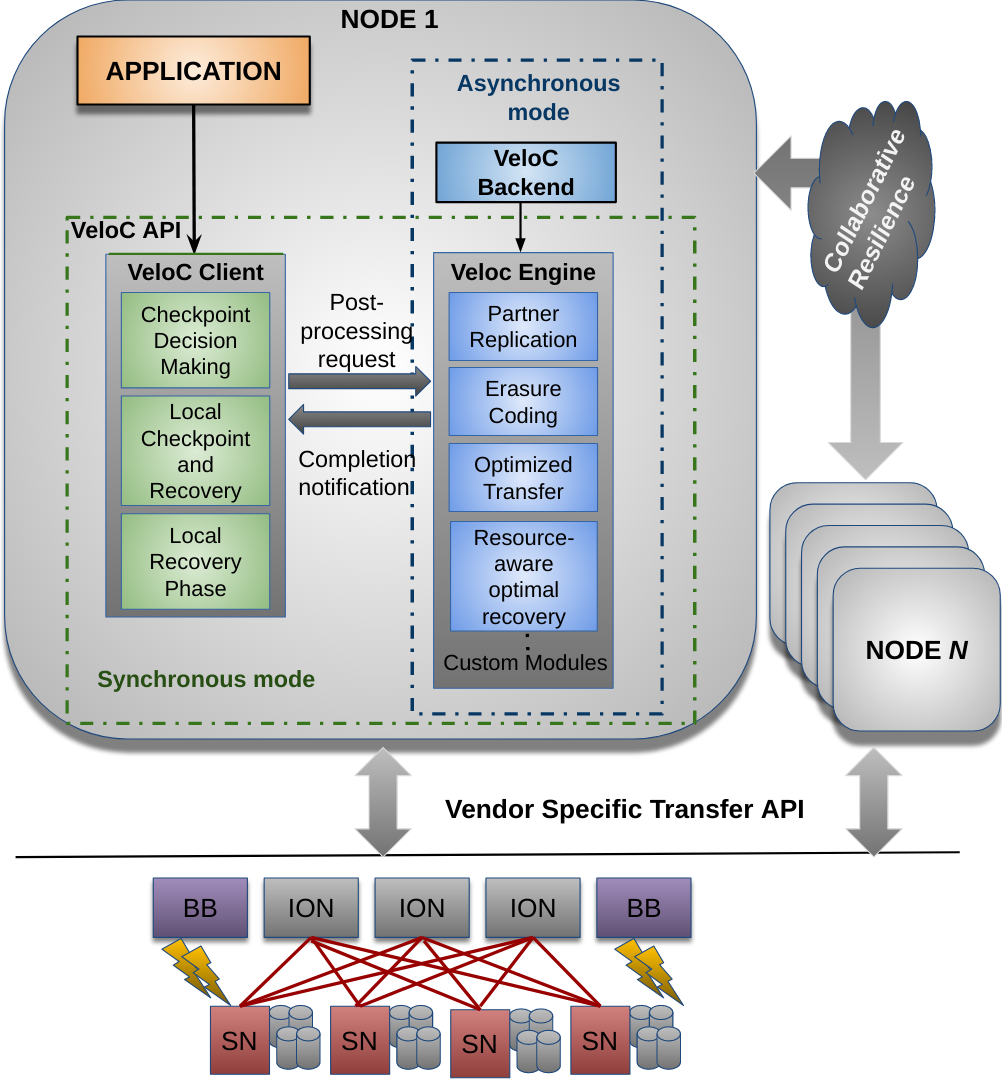
\includegraphics[width=0.47\textwidth]{projects/2.3.4-DataViz/2.3.4.05-VeloC/veloc-arch}
  \caption{VeloC: Architecture}%
  \label{fig:veloc:arch}%
\end{wrapfigure}


\begin{figure}[t]
  \begin{subfloat}[HACC\label{fig:veloc:hacc}]
  \centering
  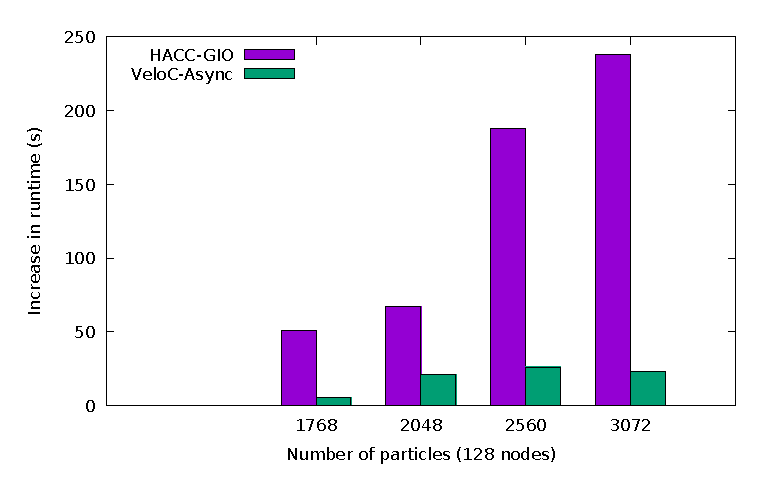
\includegraphics[width=.47\textwidth]{projects/2.3.4-DataViz/2.3.4.05-VeloC/veloc-hacc}
  \end{subfloat}
  \hfill
  \begin{subfloat}[LatticeQCD\label{fig:veloc:lqcd}]
  \centering
  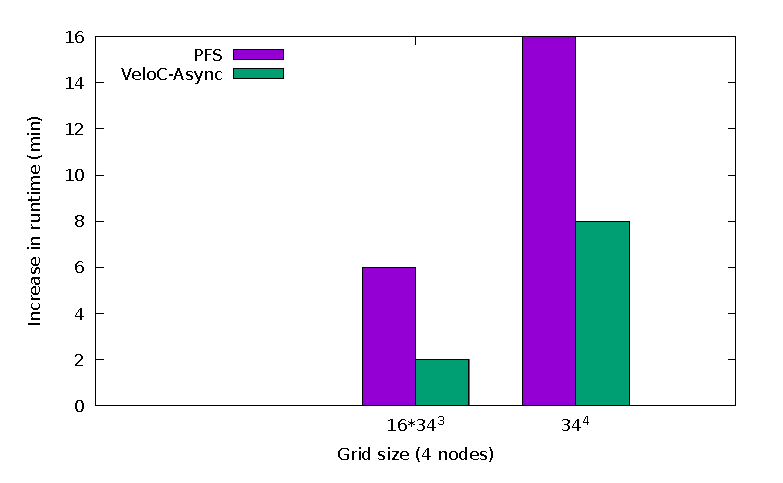
\includegraphics[width=.47\textwidth]{projects/2.3.4-DataViz/2.3.4.05-VeloC/veloc-lqcd}
  \end{subfloat}
  \caption{VeloC results with ECP applications: increase in execution time due to checkpointing (lower is better)}
  \label{fig:veloc:results}%
\end{figure}

We have evaluated VeloC with two representative use cases from the
HACC and LatticeQCD teams. The experiments were performed on the
ANL Theta platform (KNL nodes, local SSD, Lustre parallel file system).
We compared checkpointing using VeloC in asynchronous mode vs. the
original checkpointing mechanism used by the application (GenericIO
for HACC, direct writes to the parallel file system for LatticeQCD).
Results are shown in Figure~\ref{fig:veloc:results}: the impact
of checkpointing (measured as increase in runtime vs. the case
when no checkpointing is used) was reduced by up to 10x when using
VeloC.

We are also interacting with ALCF to understand the constraints for
VeloC deployment on CORAL systems, such as the configuration of the
resource and job manager and the possibility to run two MPI executions
(application + backend) on each node.

We integrated VeloC with the rest of the ECP ecosystem as well. Specifically,
we have created a Spack installation package and have facilitated its
integration in the OpenHPC distribution.

We created an SCR-to-VeloC translation library that enables existing
SCR applications to run on the VeloC library.  This is posted
in the ECP-VeloC repository and is now available to external SCR users.

Finally we expanded the documentation and created tutorials that were
presented at various international venues to raise awareness about
VeloC within the broader HPC community at international level.

\paragraph{Next Steps}

As a next step, we are working towards two goals. First, we plan to
evaluate VeloC with the ECP applications at larger scale to validate
correctness and fix potential bottlenecks and performance issues.
Based on these findings, we will improve VeloC and prepare for the
next release. In parallel, we will continue to collaborate with the
application teams to address new requirements should they arise.
Furthermore, we will expand our user base beyond ECP to interact and
get feedback from the broader international community.
